\documentclass[11pt,a4paper,english]{article}
\usepackage[english]{babel} % Using babel for hyphenation
\usepackage{lmodern} % Changing the font
\usepackage[utf8]{inputenc}
\usepackage[T1]{fontenc}

%\usepackage[moderate]{savetrees} % [subtle/moderate/extreme] really compact writing
\usepackage{tcolorbox}
\tcbuselibrary{hooks}
\usepackage[parfill]{parskip} % Removes indents
\usepackage{amsmath} % Environment, symbols etc...
\usepackage{amssymb}
\usepackage{framed}
\usepackage{float} % Fixing figure locations
\usepackage{multirow} % For nice tables
%\usepackage{wasysym} % Astrological symbols
\usepackage{graphicx} % For pictures etc...
\usepackage{enumitem} % Points/lists
\usepackage{physics} % Typesetting of mathematical physics examples: 
                     % \bra{}, \ket{}, expval{}
\usepackage{url}
\usepackage{mathtools}
\usepackage{graphicx}
\usepackage{caption}
\usepackage{subcaption}
\newenvironment{algorithm}{%
\refstepcounter{algcounter}
\begin{tcolorbox}
\centerline{Algorithm \thealgcounter}\vspace{2mm}
}
{\end{tcolorbox}}


% To include code(-snippets) with æøå
\usepackage{listings}


\tolerance = 5000 % Bedre tekst
\hbadness = \tolerance
\pretolerance = 2000

\numberwithin{equation}{section}

\definecolor{red}{RGB}{255,20,147}

\newcommand{\conj}[1]{#1^*}
\newcommand{\ve}[1]{\mathbf{#1}} % Vektorer i bold
\let\oldhat\hat
\renewcommand{\hat}[1]{\oldhat{#1}}
\newcommand{\trans}[1]{#1^\top}
\newcommand{\herm}[1]{#1^\dagger}
%\renewcommand{\thefootnote}{\fnsymbol{footnote}} % Gir fotnote-symboler
\newcommand{\Real}{\mathbb{R}}
\newcommand{\bigO}[1]{\mathcal{O}\left( #1 \right)}

%\renewcommand{\thesection}{\Roman{section}} 
%\renewcommand{\thesubsection}{\thesection.\Roman{subsection}}

\newcommand{\spac}{\hspace{5mm}}

\newcounter{algcounter}
\newcommand{\algnum}{\stepcounter{algcounter}\Roman{algcounter}}

\title{MEK4250\\Mandatory assignment 2}
\author{Krister Stræte Karlsen}
\date{\today}

\begin{document}
\tcbset{before app=\parfillskip0pt}
\maketitle

The programs belonging to this assignment is available at \\
\texttt{\color{red}{https://github.com/krikarls/MEK4250}}

\section{Stokes equation}

\subsection{Analysis of the weak formulation (Exercise 7.1)}

In this exercise we want to show some of the properties that must be satisfied in order to have a well posed Stokes problem using a mixed formulation: $u,v \in V = H^1$, $p,q \in Q = L_2 = H_0$.

\textbf{Continuity of $a(u,v)$}

In order to establish \emph{continuity}, or \emph{boundedness}, of $a(u,v)$ we must have that 
\begin{align}
\int \nabla u : \nabla v dx \leq C||u||_1 ||v||_1.
\end{align}
We square both sides
\begin{align}
\left( \int \nabla u : \nabla v dx \right)^2 \leq \left( C||u||_1 ||v||_1 \right)^2
\end{align}
and claim that if (1.2) holds, so does (1.1). Next we apply \emph{Cauchy-Schwartz'}: 
\begin{align*}
\left( \int \nabla u : \nabla v dx \right)^2 &\leq ||\nabla u||_0^2 ||\nabla v||_0^2 \\
&\leq 2||\nabla u||_0^2 ||\nabla v||_0^2 + 2||\nabla u||_0^2 ||v||_0^2 + 2||u||_0^2 ||\nabla v||_0^2 +2||u||_0^2 ||v||_0^2 \\
&= 2 \left( ||u||_0^2 + ||\nabla u||_0^2  \right) \left( ||v||_0^2 + ||\nabla v||_0^2  \right) \\
&= C ||u||_1^2 ||v||_1^2
\end{align*} 
We are now happy and move on to show continuity of $b(u,q)$.

\newpage

\textbf{Continuity of $b(u,q)$}

For continuity of $b(u,q)$ it is required that
\begin{align*}
\int q(\nabla \cdot u) dx \leq C ||u||_1 ||q||_0.
\end{align*}
Using \emph{Cauchy-Schwartz'} 
\begin{align*}
\int q(\nabla \cdot u) dx \leq ||q||_0 ||\nabla \cdot u ||_0. 
\end{align*}
we realize that if  
\begin{align*}
||\nabla \cdot u||_0 \leq  C ||u||_1.
\end{align*}
holds we are on safe ground. Without any worries(since both sides are positive) both sides can be squared. 
\begin{align*}
||\nabla \cdot u||_0^2 &\leq  ||u||_1^2 \\
&=  \left( ||u||_0 + ||\nabla u ||_0  \right) \\
&\leq \left( (D|u|_1)^2 + ||\nabla u||_0^2  \right) \\
&=  \left( (D||\nabla u||_0)^2 + ||\nabla u||_0^2  \right) \\
&= (D^2+1)||\nabla u||_0^2
\end{align*}

It is now sufficient to show that if $||\nabla \cdot u||_0^2 \leq D_2|| \nabla u||_0^2$ holds we have boundedness of $b(u,q)$. We start by writing out both terms(here assuming 2D): 
\begin{align*}
||\nabla \cdot u||_0^2 &= \int \left( \frac{\partial u_1}{\partial x} + \frac{\partial u_2}{\partial y}\right)^2 dx \\ 
|| \nabla u||_0^2 &= \int \left( \frac{\partial u_1}{\partial x} \right)^2 + \left( \frac{\partial u_2}{\partial x} \right)^2 + \left( \frac{\partial u_1}{\partial y} \right)^2 + \left( \frac{\partial u_2}{\partial y} \right)^2 dx
\end{align*}
One can now see that by adding some carefully chosen positive terms to $||\nabla \cdot u||_0^2$ we obtain 
$|| \nabla u||_0^2$, which ensures that $||\nabla \cdot u||_0^2$ must be smaller.
\begin{align*}
||\nabla \cdot u||_0^2 &\leq \int \left( \frac{\partial u_1}{\partial x} + \frac{\partial u_2}{\partial y} \right)^2 + \left( \frac{\partial u_1}{\partial x} - \frac{\partial u_2}{\partial y} \right)^2 + 2\left( \frac{\partial u_2}{\partial x} \right)^2 + 2\left( \frac{\partial u_1}{\partial y} \right)^2  dx \\ 
&= 2 \int \left( \frac{\partial u_1}{\partial x} \right)^2 + \left( \frac{\partial u_2}{\partial x} \right)^2 + \left( \frac{\partial u_1}{\partial y} \right)^2 + \left( \frac{\partial u_2}{\partial y} \right)^2 dx \\
&= D_ 2 || \nabla u||_0^2
\end{align*}


 
\newpage

\textbf{Coersivity of $a(u,q)$}

Coersivity of $a(u,q)$ is established if the following inequality is fulfilled:
\begin{align*}
C||u||_1^2 \leq \int \nabla u : \nabla u dx. 
\end{align*}

We start by rewriting the left hand side and applying \emph{Poincaré}
\begin{align*}
||u||_1^2 &= ||u||_0^2 + ||\nabla u||_0^2 \\
 &\leq (D||\nabla u||_0^2)+||\nabla u||_0^2 \\
 &= (D^2+1)||\nabla u||^2_0 \\
 &=  (D^2+1)\int \nabla u : \nabla u dx
\end{align*}
$C = 1/(D^2+1)$ and we are very happy. 


\subsection{Looking into the error estimate (Exercise 7.6)}

To investigate the error estimate
\begin{align*}
||E_u||_1 + ||E_p||_0 \leq Ch^k ||u||_{k+1} + Dh^{l+1}||p||_{l+1}
\end{align*}
we define the \emph{Stokes problem}:
\begin{align*}
-\Delta \mathbf{u} + \nabla p = \mathbf{f}, \quad \mathbf{u} = sin(\pi y) \mathbf{i} + cos(\pi x) \mathbf{j}.
\end{align*}

Computing error and convergence rates for different combinations of polynomials we obtained the results below. 

\begin{table}[H]
\centering
\caption{Convergence rates for $u$ and $p$ respectively. Convergence rates for $u$ are measured in $H^1$ while rates for $p$ are measured in $L_2$.}
\vspace{3mm}
\begin{tabular}{|l|l|l|l|l|l|l|l|l|l|l|}
\hline
 \multicolumn{2}{|c|}{ $P_4-P_3$} &  \multicolumn{2}{|c|}{ $P_4-P_2$} &  \multicolumn{2}{|c|}{ $P_3-P_2$} &  \multicolumn{2}{|c|}{ $P_3-P_1$} \\
\hline
4.29515 & 4.07241 & 2.88045 & 2.91318 & 2.84922 & 2.91507 & 2.08926 & 2.17433 \\
\hline
4.11510 & 4.02557 & 2.96138 & 2.97733 & 2.95217 & 2.97799 & 2.04644 & 2.08797 \\
\hline
4.03899 & 4.00955 & 2.98766 & 2.99487 & 2.98475 & 2.99505 & 2.02451 & 2.04127 \\
\hline
\end{tabular}
\label{tab:vel}
\end{table}

From figure 1 and table 1 we see that two of the polynomial-combinations, $P_4-P_2$ and $P_3-P_2$, yields the same results. Why is that? In search of answers we turn to the error estimate for the respective combinations of elements:
\begin{align*}
P_4-P_2: \quad ||E_u||_1 + ||E_p||_0 &\leq Ch^4 ||u||_{5} + Dh^{3}||p||_{3} \\
P_3-P_2: \quad ||E_u||_1 + ||E_p||_0 &\leq Ch^3 \left( ||u||_{4} + ||p||_{3} \right)
\end{align*}
For the first error estimate, $P_4-P_2$, the dominating term on the right hand side is the one related to the pressure, because the part related to the velocity tends to zero much faster as the mesh is refined. We are in a sense limited by the order of the polynomial we have for pressure and can obtain no better convergence than for $P_3-P_2$.

The same reasoning goes for last two combinations of elements. 

\begin{figure}[h!] 
\begin{center}
  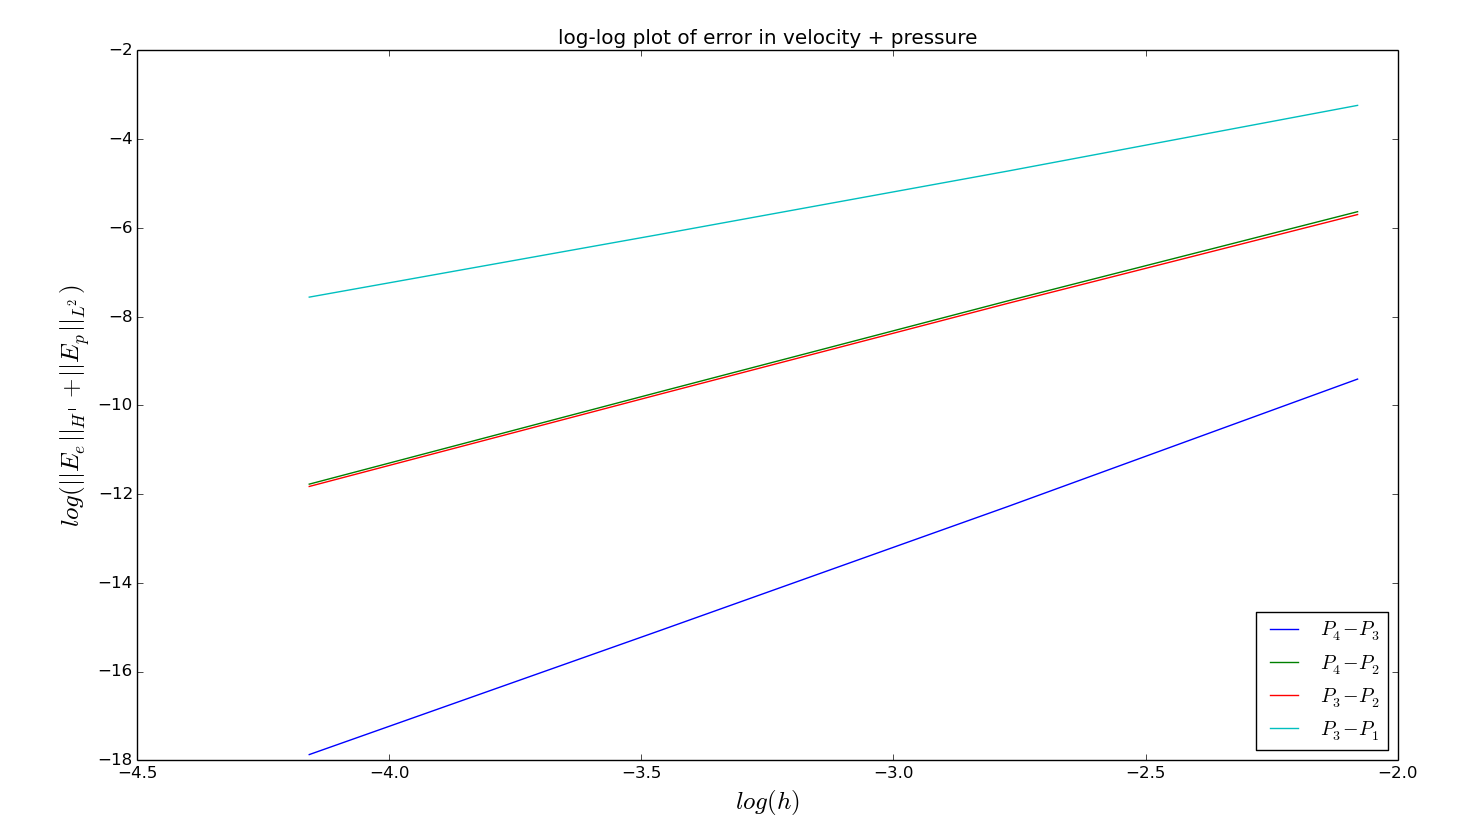
\includegraphics[scale=0.25]{stokes_loglog.png}
  \end{center}
  \caption{Log-log plot of error for different combinations of polynomials.}
   \label{fig:stokes}
\end{figure}

\subsection{Approximation of the shear stress (Exercise 7.7)}

In this section we will have a look at the order of approximation for the \emph{wall shear stress}; that is, for a wall parallel to the $x-axis$ 
\begin{align*}
\tau = \mu \frac{du}{dy}.
\end{align*}

We study this by computing the wall shear stress analytically, then numerically and last compute the error. 

\begin{table}[H]
\centering
\caption{Computed convergence rates $r_n$ using a $L^2-$norm for different combinations of polynomials. Increase in $n$ refers to refined mesh. }
\vspace{3mm}
\begin{tabular}{|l|l|l|l|l|l|l|l|l|l|l|}
\hline
 & $P_4-P_3$ & $P_4-P_2$ & $P_3-P_2$ & $P_3-P_1$ \\
\hline
$r_1$ & 4.136169 & 2.950468 & 3.025279 & 2.285654 \\
\hline
$r_2$ & 4.048773 & 2.997513 & 3.080835 & 2.148821 \\
\hline
$r_3$ & 4.021954 & 3.006015 & 3.065985 & 2.054565 \\
\hline
\end{tabular}
\label{tab:shear}
\end{table}

By looking at the convergence rates(table \ref{tab:shear}) and the log-log plot of the error(figure \ref{fig:shearstress}) one can observe that error behaves like a $H^1-$norm, even though we used a $L^2-$norm to compute the error. That should come as no surprise to the shrewd reader, as the shear stress involves the derivative of the velocity, as does the $H^1-$ norm. In other words; the results for the convergence rates here are of the same order as in the previous section(table \ref{tab:vel}) where we measured the error in velocity in $H^1$.

\begin{figure}[h!] 
\begin{center}
  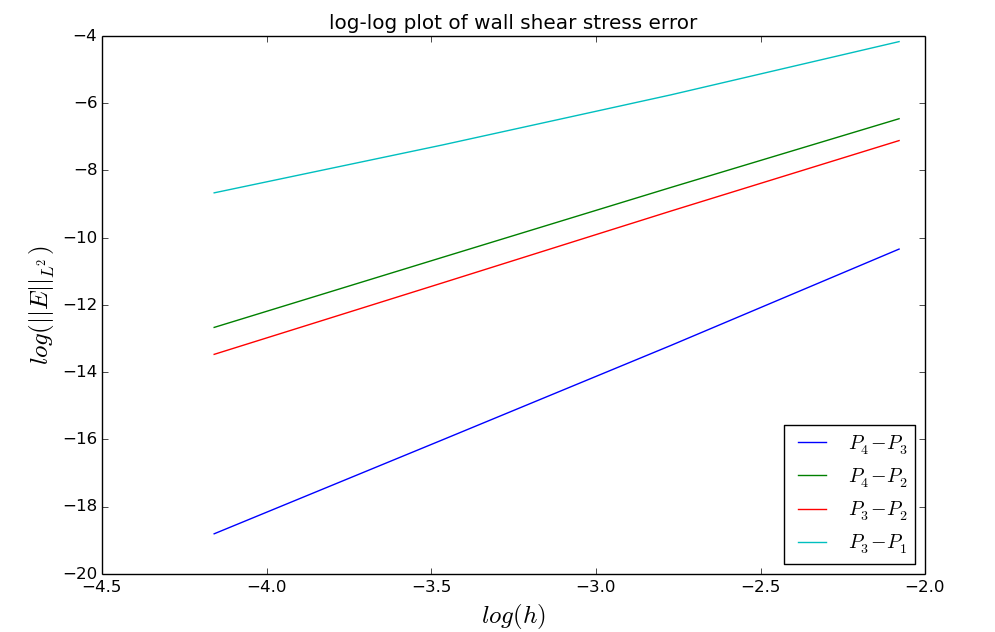
\includegraphics[scale=0.3]{shear_loglog.png}
  \end{center}
  \caption{Log-log plot of the wall shear stress error($L^2$) for different combinations of polynomials.}
   \label{fig:shearstress}
\end{figure}

\newpage


\section{Linear elasticity}

To study a phenomenon in numerical linear elasticity called \emph{locking} we look a the following problem:
\begin{align}
-\mu \Delta \mathbf{u} - \lambda \nabla \nabla \cdot \mathbf{u} = \mathbf{f} \quad &in \quad \Omega=(0,1)^2 , \\
\mathbf{u} = \left( \frac{\partial \phi}{\partial u} , -\frac{\partial \phi}{\partial x} \right) \quad &on \quad \partial \Omega ,
\end{align}
where $\phi = sin(\pi x y)$ .

We start deriving and expression for the external forces $\mathbf{f}$.

Since $\nabla \cdot \mathbf{u} = 0$ we have that $\mathbf{f} = - \mathbf{u} \Delta u$. This can be computed using \texttt{sympy} or by hand calculations, like they did in the old days. We find that:
\begin{align*}
\mathbf{f} =  \pi^2(\pi x (x^2+y^2)cos(\pi xy)+ 2y sin(\pi x y)) \mathbf{i} \\ -\pi^2(\pi y(x^2+y^2)cos(\pi xy)+2x sin(\pi xy))\mathbf{j}.
\end{align*}

Problem (2.1)-(2.2) will now be solved using finite element methods in FEniCS. Three different approaches for the $\lambda \nabla \nabla \cdot \mathbf{u}-$term will be tested and discussed. Here listed from stupid to clever:

1) Keep the $\lambda \nabla \nabla \cdot \mathbf{u}$-term as it is. \\
2) Integrate $\lambda \nabla \nabla \cdot \mathbf{u}$ by parts. \\
3) Define $p=\lambda(\nabla \cdot \mathbf{u})$ such that $\lambda \nabla \nabla \cdot \mathbf{u} = \nabla p$ and use a mixed finite element formulation. 

\textbf{Approach \#1}

We think no further, and ignore what we have learned, and implement and solve problem (2.1)-(2.2) in FEniCS as:

\begin{framed}
\texttt{a = inner(grad(u),grad(v))*dx-lmbda*inner(grad(div(u)),v)*dx \\
L = inner(f,v)*dx}  
\end{framed} 

The results obtained by this approach are very poor and can be viewed in table \ref{tab:err1} and \ref{tab:con1}. 

\begin{table}[H]
\centering
\caption{ L2-errors from using approach \#1 and second order polynomials.}
\vspace{3mm}
\begin{tabular}{|l|l|l|l|l|l|l|l|l|l|l|}
\hline
$\lambda\backslash$N & 8 & 16 & 32 & 64 \\
\hline
1 & 0.014961 & 0.003950 & 0.001002 & 0.000251 \\
\hline
10 & 0.725727 & 0.691354 & 0.026575 & 0.006363 \\
\hline
100 & 3.750028 & 0.606093 & 0.650818 & 2.416408 \\
\hline
1000 & 2.088700 & 0.823344 & 1.165615 & 0.514192 \\
\hline
10000 & 1.426623 & 1.681094 & 3.957783 & 1.143778 \\
\hline
\end{tabular}
\label{tab:err1}
\end{table}

\begin{table}[H]
\centering
\caption{ Convergence-rates using approach \#1 and second order polynomials. }
\vspace{3mm}
\begin{tabular}{|l|l|l|l|l|l|l|l|l|l|l|}
\hline
$\lambda \backslash$N & $r_1$ & $r_2$ & $r_3$ \\
\hline
1 & 1.921346 & 1.979257 & 1.994746 \\
\hline
10 & 0.070003 & 4.701297 & 2.062245 \\
\hline
100 & 2.629290 & -0.102715 & -1.892538 \\
\hline
1000 & 1.343039 & -0.501525 & 1.180714 \\
\hline
10000 & -0.236797 & -1.235292 & 1.790886 \\
\hline
\end{tabular}
\label{tab:con1}
\end{table}


So what is happening? 

We can definitely see that when $\lambda$ gets bigger the numerical solution is bad. Only for $\lambda=1$ are the results reasonable. The convergence rates are in this case stable, but lower than expected. If we plot and compare the solutions we see that the deformations/displacements computed numerically are less then they should be. One might even say that the deformation seems to be \emph{"locked"}, see figure \ref{fig:locking}.

\begin{figure}[h!] 
\begin{center}
  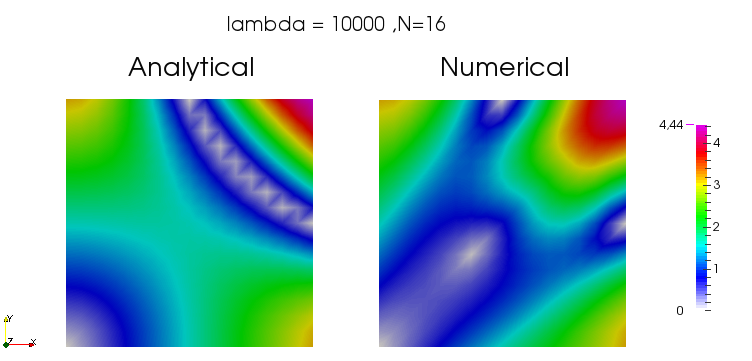
\includegraphics[scale=0.4]{locking.png}
  \end{center}
  \caption{Comparing analytical and numerical solution for approach \#1.}
  \label{fig:locking}
\end{figure}

This is because we use elements that approximate the divergence poorly and when that term of the equation starts to dominate things fall apart. This phenomenon is called \emph{locking.} 

\textbf{Approach \#2}

Now, let's integrate the bad term by parts and see what happens. The variational formulation now reads:

\begin{framed} 
\texttt{a = inner(grad(u),grad(v))*dx+lmbda*inner(div(u),div(v))*dx \\
L = inner(f,v)*dx}
\end{framed}

\begin{table}[H]
\centering
\caption{ L2-errors from using approach \#2 and second order polynomials. }
\vspace{3mm}
\begin{tabular}{|l|l|l|l|l|l|l|l|l|l|l|}
\hline
$\lambda \backslash$N & 8 & 16 & 32 & 64 \\
\hline
1 & 2.080473e-03 & 2.52145e-04 & 3.12446e-05 & 3.89691e-06 \\
\hline
10 & 3.510135e-03 & 3.24355e-04 & 3.40039e-05 & 3.98917e-06 \\
\hline
100 & 1.439727e-02 & 1.49814e-03 & 1.19452e-04 & 8.74370e-06 \\
\hline
1000 & 2.699475e-02 & 5.14354e-03 & 6.89956e-04 & 6.37015e-05 \\
\hline
10000 & 2.989324e-02 & 7.17495e-03 & 1.57723e-03 & 2.72196e-04 \\
\hline
\end{tabular}
\end{table}

\begin{figure}[h!] 
\begin{center}
  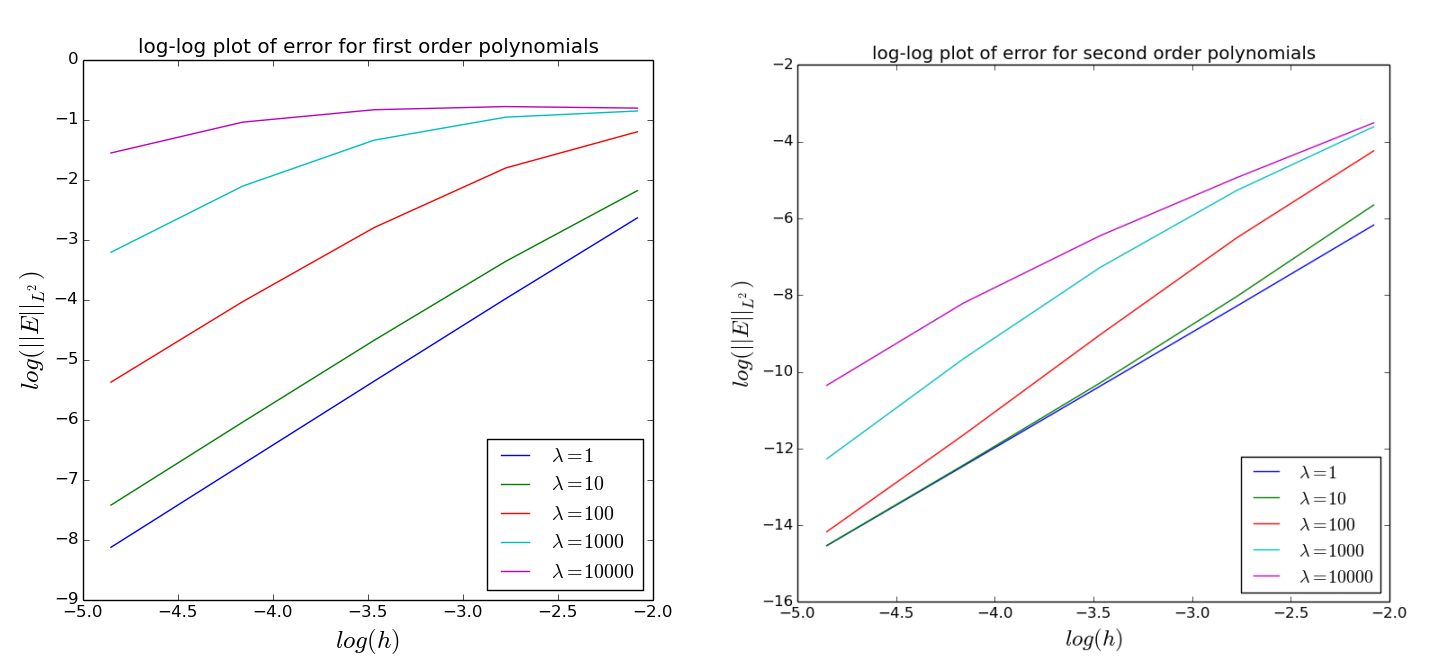
\includegraphics[scale=0.25]{LE1.png}
  \end{center}
  \caption{Log-log plot of error for first and second order polynomials for approach \#2.}
\end{figure}


\begin{table}[H]
\centering
\caption{Convergence-rates using approach \#2 and second order polynomials. }
\vspace{3mm}
\begin{tabular}{|l|l|l|l|l|l|l|l|l|l|l|}
\hline
$\lambda \backslash$N & $r_1$ & $r_2$ & $r_3$ \\
\hline
1 & 3.044586 & 3.01258 & 3.00320 \\
\hline
10 & 3.435881 & 3.25380 & 3.09154 \\
\hline
100 & 3.264555 & 3.64867 & 3.77204 \\
\hline
1000 & 2.391844 & 2.89819 & 3.43711 \\
\hline
10000 & 2.058779 & 2.18558 & 2.53468 \\
\hline
\end{tabular}
\end{table}

The solution has now improved, but that are still some problems. For $\lambda=1$ everything works fine, the error decreases, the convergence rates are stable and of the expected order. For $\lambda \geq 10$ we can see fluctuations in the convergence rate, even though the $L_2-$errors are fairly low. 

Next; let's try to be really clever!

\textbf{Approach \#3: Stabilization using a mixed finite element formulation}

We define $p=\lambda(\nabla \cdot \mathbf{u})$ such that $\lambda \nabla \nabla \cdot \mathbf{u} = \nabla p$. Problem (2.1)-(2.2) can then be formulated
\begin{align*}
-\mu \Delta \mathbf{u} - \nabla p = \mathbf{f}, \\ 
(\nabla \cdot \mathbf{u}) - \frac{1}{\lambda} p, = 0
\end{align*}
with the weak formulation 
\begin{align*}
\int_\Omega \nabla \mathbf{u} : \nabla \mathbf{v} dx + \int_\Omega p(\nabla \cdot \mathbf{v}) dx = \int_\Omega \mathbf{f} \cdot \mathbf{v} dx \quad \forall \mathbf{v}\in V,  \\
\int_\Omega (\nabla \cdot \mathbf{u})q dx - \frac{1}{\lambda} \int_{\Omega} pq dx = 0 \quad \forall q \in Q. 
\end{align*}

We implement this in FEniCS and look at the results with a happy face. 

\begin{framed}
\texttt{	a = inner(grad(u),grad(v))*dx + div(v)*p*dx \\
	a2 = q*div(u)*dx - (1.0/lmbda)*p*q*dx \\
	 L = inner(f,v)*dx  }
\end{framed}

\begin{table}[H]
\centering
\caption{ L2-errors using a mixed FEM formulation $P_2 -P_1$. }
\vspace{3mm}
\begin{tabular}{|l|l|l|l|l|l|l|l|l|l|l|}
\hline
$\lambda \backslash$N & 8 & 16 & 32 & 64 \\
\hline
1 & 1.987451e-03 & 2.48875e-04 & 3.11388e-05 & 3.89358e-06 \\
\hline
10 & 1.968511e-03 & 2.48207e-04 & 3.11171e-05 & 3.89289e-06 \\
\hline
100 & 1.971773e-03 & 2.48317e-04 & 3.11211e-05 & 3.89304e-06 \\
\hline
1000 & 1.973119e-03 & 2.48367e-04 & 3.11230e-05 & 3.89311e-06 \\
\hline
10000 & 1.973277e-03 & 2.48373e-04 & 3.11233e-05 & 3.89312e-06 \\
\hline
\end{tabular}
\end{table}

\begin{table}[H]
\centering
\caption{ Convergence-rates using a mixed FEM formulation $P_2 -P_1$.}
\vspace{3mm}
\begin{tabular}{|l|l|l|l|l|l|l|l|l|l|l|}
\hline
$\lambda \backslash$N & $r_1$ & $r_2$ & $r_3$ \\
\hline
1 & 2.997423 & 2.99864 & 2.99955 \\
\hline
10 & 2.987488 & 2.99577 & 2.99879 \\
\hline
100 & 2.989240 & 2.99621 & 2.99892 \\
\hline
1000 & 2.989934 & 2.99642 & 2.99899 \\
\hline
10000 & 2.990015 & 2.99644 & 2.99899 \\
\hline
\end{tabular}
\end{table}

Our results are now very satisfactory. The numerical solution is now unaffected by the size of $\lambda$. We have successfully avoided \emph{locking}.  


\end{document}
